\documentclass[12pt]{article}

\usepackage{listings}
\usepackage{graphicx}
\usepackage{float}
\usepackage{hyperref}

\usepackage{amssymb} 
\usepackage{amsmath}
\usepackage{amsthm}
\usepackage{sansmath}
\usepackage{epsfig}

\usepackage[T1]{fontenc}
\usepackage{lmodern}
\renewcommand*\familydefault{\sfdefault}

\usepackage[margin=2cm]{geometry}

\usepackage[parfill]{parskip}
\linespread{1.2} 

\usepackage{xcolor}

\lstdefinestyle{code}{  
    commentstyle=\color{gray},
    keywordstyle=\color{blue},
    numberstyle=\tiny\color{gray},
    stringstyle=\color{teal},
    ndkeywordstyle=\color{purple},
    basicstyle=\ttfamily\footnotesize,
    breakatwhitespace=false,         
    breaklines=true,                 
    captionpos=t,                    
    keepspaces=true,                 
    numbers=left,                    
    numbersep=8pt,                  
    showspaces=false,                
    showstringspaces=false,
    showtabs=false,                  
    tabsize=4,
    frame=single,
    breaklines=true
}

\lstset{style=code}

\newcounter{question}
\setcounter{question}{0}
\newcounter{subquest}

\newcommand{\question}[1]{
    \stepcounter{question} 
    \vspace{1em}
    \textbf{\Large\thequestion \ - #1}
    \vspace{.5em} 
    \setcounter{subquest}{0}\ \\}

\newcommand{\subquestion}{
    \stepcounter{subquest} 
    \vspace{.5em}
    \textbf{\large Question \thequestion.\thesubquest}
    \vspace{.25em}\ \\}

\newcommand{\solution}
    {\par\vspace{0.5em}\noindent\emph{Solution.}\ }
    {\par\vspace{1em}}

\usepackage{fancyhdr}
\setlength{\headheight}{15pt}
\pagestyle{fancy} 
\lhead{Math 5334: \emph{Numerical Analysis}}
\rhead{Serena Su}
\cfoot{}
\rfoot{\thepage}

\begin{document}

\begin{center}
\textbf{\huge Homework 3}

{\large\emph{Due Date: October 27, 2025}}
\vspace{1em}
\end{center}
\hrule

\question{Hermite Interpolation}

Given the function 
\[f(x)=\frac{1}{1+25x^2}, \quad x\in[-1,1],\]
with the function values and first derivatives at the nodes 
\[x_0=-1, \quad x_1=0, \quad x_2=1 \]

\subquestion
Construct the cubic Hermite interpolant $H(x)$ and evaluate $H(0.5)$.

\solution
The cubic Hermite interpolant on an interval $[x_0, x_{1}]$ is determined by the shape functions:
\[h_{00}(t) = 2t^3 - 3t^2 + 1, \quad h_{01}(t) = -2t^3 + 3t^2\]
\[h_{10}(t) = t^3 - 2t^2 + t, \quad h_{11}(t) = t^3 - t^2\]
Provided $h=x_1-x_0$ and $t=\frac{x-x_0}{h} \in [0,1]$. 
The cubic Hermite interpolant is given by:
\[H(x) = f(x_0)h_{00}(t) + f(x_1)h_{01}(t) + h\left[f'(x_0)h_{10}(t) + f'(x_1)h_{11}(t)\right]\]

We will construct the Hermite interpolant piecewise on the intervals $[-1,0]$ and $[0,1]$.

To start off with, the following table summarizes the function and derivative values at the nodes:
\begin{center}
\begin{tabular}{|c|c|c|}
\hline
Node $x_j$ & $f(x_j)$ & $f'(x_j)$ \\
\hline
-1 & $\frac{1}{26}$ & $\frac{50}{676} = \frac{25}{338}$ \\
0 & 1 & 0 \\
1 & $\frac{1}{26}$ & $-\frac{25}{338}$ \\
\hline
\end{tabular}
\end{center}
Where $f'(x)=\frac{-50x}{(1+25x^2)^2}$.

On $[-1,0]$, we have $h=1$ and $t=x+1$. So therefore we have:
\[h_{00}(x+1) = 2(x+1)^3 - 3(x+1)^2 + 1 = 2x^3 + 3x^2\]
\[h_{01}(x+1) = -2(x+1)^3 + 3(x+1)^2 = -2x^3 - 3x^2 + 1\]
\[h_{10}(x+1) = (x+1)^3 - 2(x+1)^2 + (x+1) = x^3 + x^2\]
\[h_{11}(x+1) = (x+1)^3 - (x+1)^2 = x^3+2x^2+x\]

Substituting into the interpolant formula, we get:
\[H(x) = \frac{1}{26}(2x^3 + 3x^2) + 1(-2x^3 - 3x^2 + 1) + 1 \cdot \frac{25}{338}(x^3 + x^2) + 0\]
Simplifying, we have:
\[H(x) = -\frac{625}{338}x^3 - \frac{475}{169}x^2 + 1, \quad x\in[-1,0]\]

On $[0,1]$, we have $h=1$ and $t=x$. So therefore our shape functions are as defined initially with $x$ in place of $t$.
Substituting into the interpolant formula, we get:
\[H(x) = 1(2x^3 - 3x^2 + 1) + \frac{1}{26}(-2x^3 + 3x^2) + 0 -\frac{25}{338}(x^3 - x^2)\]
Simplifying, we have:
\[H(x) = \frac{625}{338}x^3 - \frac{475}{169}x^2 + 1, \quad x\in[0,1]\]

So the cubic Hermite interpolant is:
\[H(x) = \begin{cases} -\frac{625}{338}x^3 - \frac{475}{169}x^2 + 1, & x\in[-1,0] \\[6pt] \frac{625}{338}x^3 - \frac{475}{169}x^2 + 1, & x\in[0,1] \end{cases}\]

Evaluating at $x=0.5$, we get that:
\[H(0.5) = \frac{625}{338}(0.5)^3 - \frac{475}{338}(0.5)^2 + 1 = \frac{1429}{2704} \approx 0.528479290\]

\subquestion
Evaluate the absolution error of $f(0.5)-H(0.5)$, and show that the error agrees the prior estimate of 
\[f(x)-p(x)=\frac{f^{(2n+2)}(\xi)}{(2n+2)!}\prod_{j=0}^{n}(x-x_j)^2\]
for some $\xi$ between $x$ and $x_j$.

\solution
Note that $f(0.5) = \frac{4}{29} \approx 0.1379310345$. 

The absolute error with our estimate $H(0.5)$ is:
\[|f(0.5)-H(0.5)| = \left|\frac{4}{29} - \frac{1429}{2704}\right| = \frac{30625}{78416} \approx 0.390548\]
The fourth \href{https://www.derivative-calculator.net/}{derivative} of $f(x)$ is:
\[f^{(4)}(x) = \frac{15000 \left(3125x^{4} - 250x^{2} + 1\right)}{\left(25x^{2} + 1\right)^{5}}\]
The \href{https://www.wolframalpha.com/input?i=maximum+calculator&assumption=%7B%22F%22%2C+%22GlobalMaximizeCalculator%22%2C+%22curvefunction%22%7D+-%3E%22abs%2815000%283125x%5E4-250x%5E2%2B1%29%2F%28%2825x%5E2%2B1%29%5E5%29%29%22&assumption=%7B%22F%22%2C+%22GlobalMaximizeCalculator%22%2C+%22domain%22%7D+-%3E%22-1+%3C%3D+x+%3C%3D+1%22}{maximum} of $|f^{(4)}(\xi)|$ for $\xi \in [-1,1]$ occurs at $x=0$, yielding:
\[|f^{(4)}(0)| = 15000\]

The product term evaluated at $x=0.5$ is:
\[\prod_{j=1}^{2}(0.5 - x_j)^2 = (0.5 - 0)^2 (0.5 - 1)^2 = \left(\frac{1}{2}\right)^2 \cdot \left(-\frac{1}{2}\right)^2 = \frac{1}{4} \cdot \frac{1}{4} = \frac{1}{16}\]
We also have that $(2n+2)! = 4! = 24$ for $n=1$.
So putting everything together, we can estimate the error as:
\[\left|f(0.5)-H(0.5)\right| \leq \frac{15000}{24} \cdot \frac{1}{16} = \frac{625}{16} \approx 39.0625\]
So therefore our absolute error is well within the established bound.

\underbar{Extra: Absolute Error with Standard Hermite Interpolant}

\emph{Note: Question 1.1 was originally done by hand with the regular Hermite Interpolant resulting in a polynomial of degree 5. This was the error analysis conducted for that version.}

The absolute error with our estimate $P_5(0.5)$ is:
\[|f(0.5)-P_5(0.5)| = \left|\frac{4}{29} - \frac{6341}{10816}\right| = \frac{140625}{313664} \approx 0.4483300602\]

To estimate the error using the provided formula, we first need to compute the \href{https://www.derivative-calculator.net/}{sixth derivative} of $f(x)$, which works out to:
\[f^{(6)}(x) = \frac{11250000 \left(109375x^{6} - 21875x^{4} + 525x^{2} - 1\right)}{\left(25x^{2} + 1\right)^{7}}\]


The \href{https://www.wolframalpha.com/input?i=maximum+calculator&assumption=%7B%22F%22%2C+%22GlobalMaximizeCalculator%22%2C+%22curvefunction%22%7D+-%3E%22abs%2811250000%28109375x%5E6-21875x%5E4%2B525x%5E2-1%29%2F%28%2825x%5E2%2B1%29%5E7%29%29%22&assumption=%7B%22F%22%2C+%22GlobalMaximizeCalculator%22%2C+%22domain%22%7D+-%3E%22-1+%3C%3D+x+%3C%3D+1%22}{maximum} of $|f^{(6)}(\xi)|$ for $\xi \in [-1,1]$ occurs at $x=0$, yielding:
\[|f^{(6)}(0)| = 11250000\]

The product term evaluated at $x=0.5$ is:
\[\prod_{j=0}^{2}(0.5 - x_j)^2 = (0.5 + 1)^2 (0.5 - 0)^2 (0.5 - 1)^2 = \left(\frac{3}{2}\right)^2 \cdot \left(\frac{1}{2}\right)^2 \cdot \left(-\frac{1}{2}\right)^2 = \frac{9}{4} \cdot \frac{1}{4} \cdot \frac{1}{4} = \frac{9}{64}\]

We also have that $(2n+2)! = 6! = 720$ for $n=2$.

So putting everything together, we can estimate the error as:
\[\left|f(0.5)-P_5(0.5)\right| \leq \frac{11250000}{720} \cdot \frac{9}{64} = \frac{140625}{64} \approx 2197.265625\]

So therefore our absolute error is well within the established bound.

\subquestion
Obtain the cubic Hermite interpolant in Newton form $P(x)$., by constructing the Hermite divided-difference table.

\solution
The code for Lagrange Interpolation from the previous assignment was modified compute the Hermite Interpolation:
\begin{lstlisting}[language=Python, caption=1.3 Python]
import numpy as np

def f(x):
    return 1 / (1 + 25 * x**2)

def f_prime(x):
    return -50 * x / (1 + 25 * x**2)**2

def hermite_coefficients(nodes, f=f, f_prime=f_prime):
    # Parameterize nodes for Hermite interpolation
    z = np.concatenate((nodes, nodes))
    sorted_indexes = z.argsort()
    z = z[sorted_indexes]
    num_nodes = len(z)
    
    # Set up dd table with zeroth dd
    dd_table = np.array([[f(zi) for zi in z]])

    # First divided difference
    f_prime_nodes = np.array([f_prime(xi) for xi in nodes])
    zeros = np.zeros(len(nodes))
    first_dd = np.concatenate((f_prime_nodes, zeros))[sorted_indexes]
    for j in range(num_nodes - 1):
        if j % 2 == 1:
            first_dd[j] = (dd_table[0, j + 1] - dd_table[0, j]) / (z[j + 1] - z[j])
    dd_table = np.vstack([dd_table, first_dd])
    
    # Remaining Divided Differences
    for i in range(2, num_nodes):
        ith_dd = np.zeros(num_nodes)
        
        for j in range(num_nodes - i):
            # Calculate ith divided differences
            ith_dd[j] = (dd_table[i - 1, j + 1] - dd_table[i - 1, j]) / (z[j + i] - z[j])
        
        dd_table = np.vstack([dd_table, ith_dd])

    coefficients = np.array([dd_table[i, 0] for i in range(dd_table.shape[0])])
    return coefficients, dd_table.T, z

def generate_hermite(nodes, n):
    # Get coefficients
    a = hermite_coefficients(nodes)[0]
    # Start with function and constant term
    equation = f"P_{{{2*n+1}}}(x) = {a[0]}"
    w = []
    # Build (x - xi) terms
    for xi in nodes:
        if abs(xi) <= 1e-14:
            w.append('(x)')
        elif xi < 0:
            w.append(f"(x + {abs(xi)})")
        else:
            w.append(f"(x - {xi})")
    b = ""

    # Build polynomial string
    for i in range(1, len(a)):
        for j in range(i):
            # Multiply (x - xi) terms
            b += '^2' if j%2 ==1 else w[int(j/2)]
        # Multiply (x - xi) product with current coefficient and add term
        if a[i] > 0:
            equation += f" + {a[i]}{b}"
        elif a[i] < 0:
            equation += f" - {abs(a[i])}{b}"
        b = ""

    return equation

if __name__ == '__main__':
    nodes_1 = np.array([-1,0])
    equation_1 = generate_hermite(nodes_1, 1)
    table_1, z_1 = hermite_coefficients(nodes_1)[1:3]
    
    nodes_2 = np.array([0,1])
    equation_2 = generate_hermite(nodes_1, 1)
    table_2, z_2 = hermite_coefficients(nodes_1)[1:3]
    
    equations = [equation_1,equation_2]
    tables = [table_1, table_2]
    z = [z_1,z_2]
    
    with open("./outputs_3/hermite.txt", 'w') as file:        
        for k in range(2):
            file.write(equations[k] +'\n\n')

            file.write('\\begin{center}\n')
            file.write('\\begin{tabular}{|c|c|c|c|c|c|}\n')
            file.write('\\hline\n')
            file.write('& $z_i$ & $f[z_i]$ & 1st dd. & 2nd dd. & 3rd dd. \\\\\n')
            file.write('\\hline\n')
            for i in range(tables[k].shape[0]):
                file.write(f'$z_{i}$ & ${z[k][i]}$ ')
                for j in range(tables[k].shape[1]):
                    file.write(f'& ${tables[k][i,j]:.4f}$ ')
                file.write('\\\\ \n')
            file.write('\\hline\n')
            file.write('\\end{tabular}\n')
            file.write('\\end{center}\n\n')
\end{lstlisting}

The divided-difference tables and Hermite Interpolants generated were:

On $[-1,0]$:
\begin{center}
\begin{tabular}{|c|c|c|c|c|c|}
\hline
& $z_i$ & $f[z_i]$ & 1st dd. & 2nd dd. & 3rd dd. \\
\hline
$z_0$ & $-1$ & $0.0385$ & $0.0740$ & $0.8876$ & $-1.8491$ \\ 
$z_1$ & $-1$ & $0.0385$ & $0.9615$ & $-0.9615$ & $0.0000$ \\ 
$z_2$ & $0$ & $1.0000$ & $0.0000$ & $0.0000$ & $0.0000$ \\ 
$z_3$ & $0$ & $1.0000$ & $0.0000$ & $0.0000$ & $0.0000$ \\ 
\hline
\end{tabular}
\end{center}
\begin{align*}
    P_{3}(x) &= 0.038461538461538464 + 0.07396449704142012(x + 1) \\
    &+ 0.8875739644970414(x + 1)^2 - 1.849112426035503(x + 1)^2(x)
\end{align*}

On $[0,1]$:
\begin{center}
\begin{tabular}{|c|c|c|c|c|c|}
\hline
& $z_i$ & $f[z_i]$ & 1st dd. & 2nd dd. & 3rd dd. \\
\hline
$z_0$ & $0$ & $1.0000$ & $0.0000$ & $-0.9615$ & $1.8491$ \\ 
$z_1$ & $0$ & $1.0000$ & $-0.9615$ & $0.8876$ & $0.0000$ \\ 
$z_2$ & $1$ & $0.0385$ & $-0.0740$ & $0.0000$ & $0.0000$ \\ 
$z_3$ & $1$ & $0.0385$ & $0.0000$ & $0.0000$ & $0.0000$ \\ 
\hline
\end{tabular}
\end{center}
\begin{align*}
    P_{3}(x) &= 1.0 - 0.9615384615384616(x)^2\\ 
    &+ 1.849112426035503(x)^2(x - 1)
\end{align*}

\newpage
\subquestion
Plot $f(x)$, $H(x)$ and $P(x)$ on $x\in[-1,1]$.

\solution
The following plots were generated:
\begin{center}
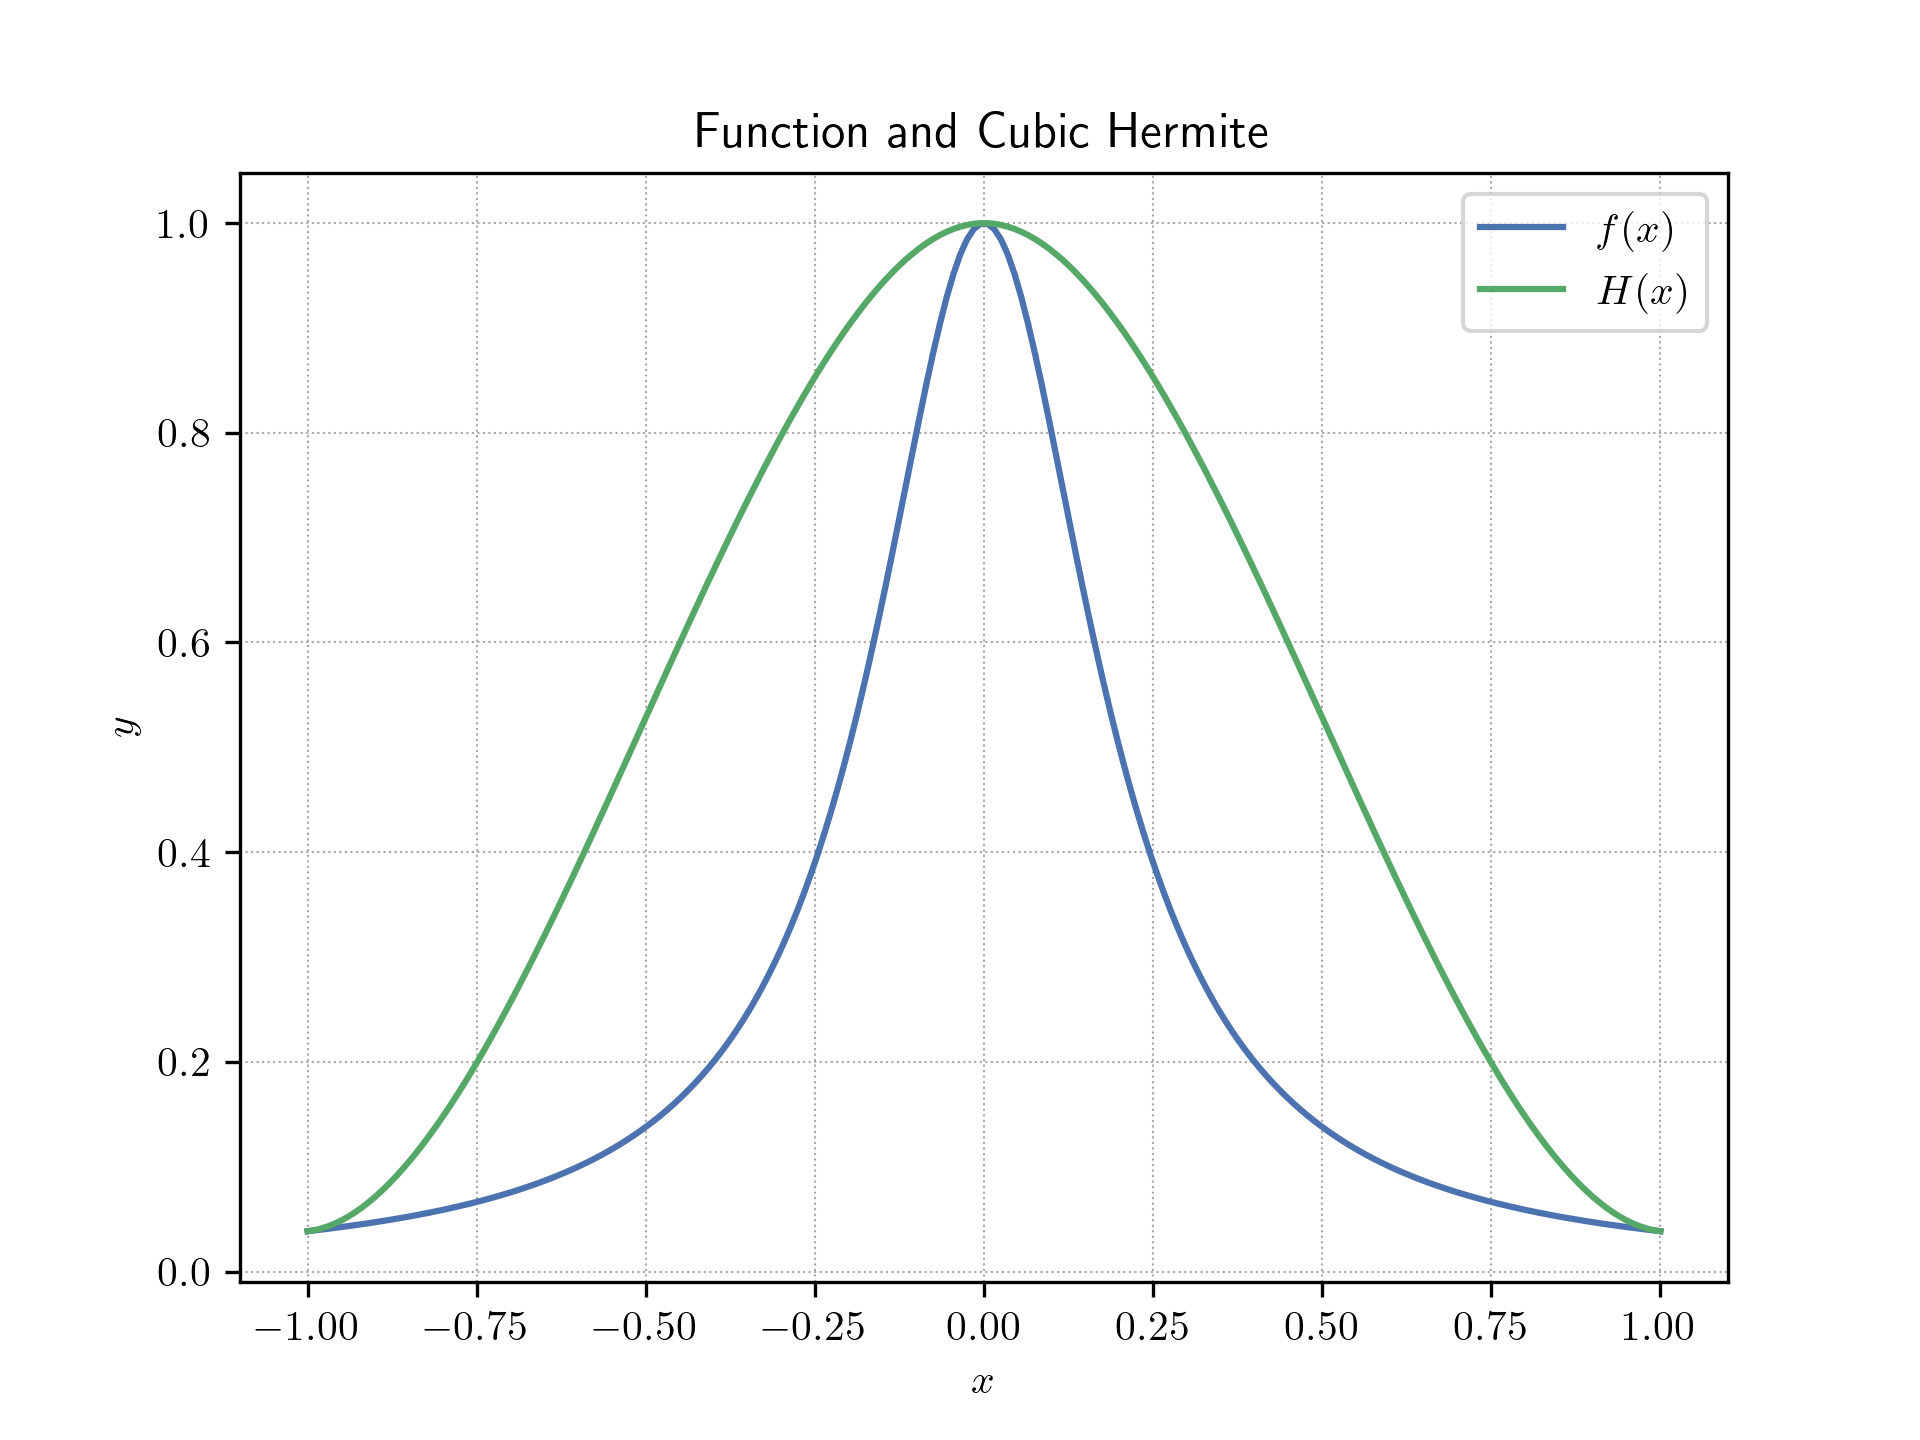
\includegraphics[width=0.7\textwidth]{../outputs_3/hermite_plot_h.png}
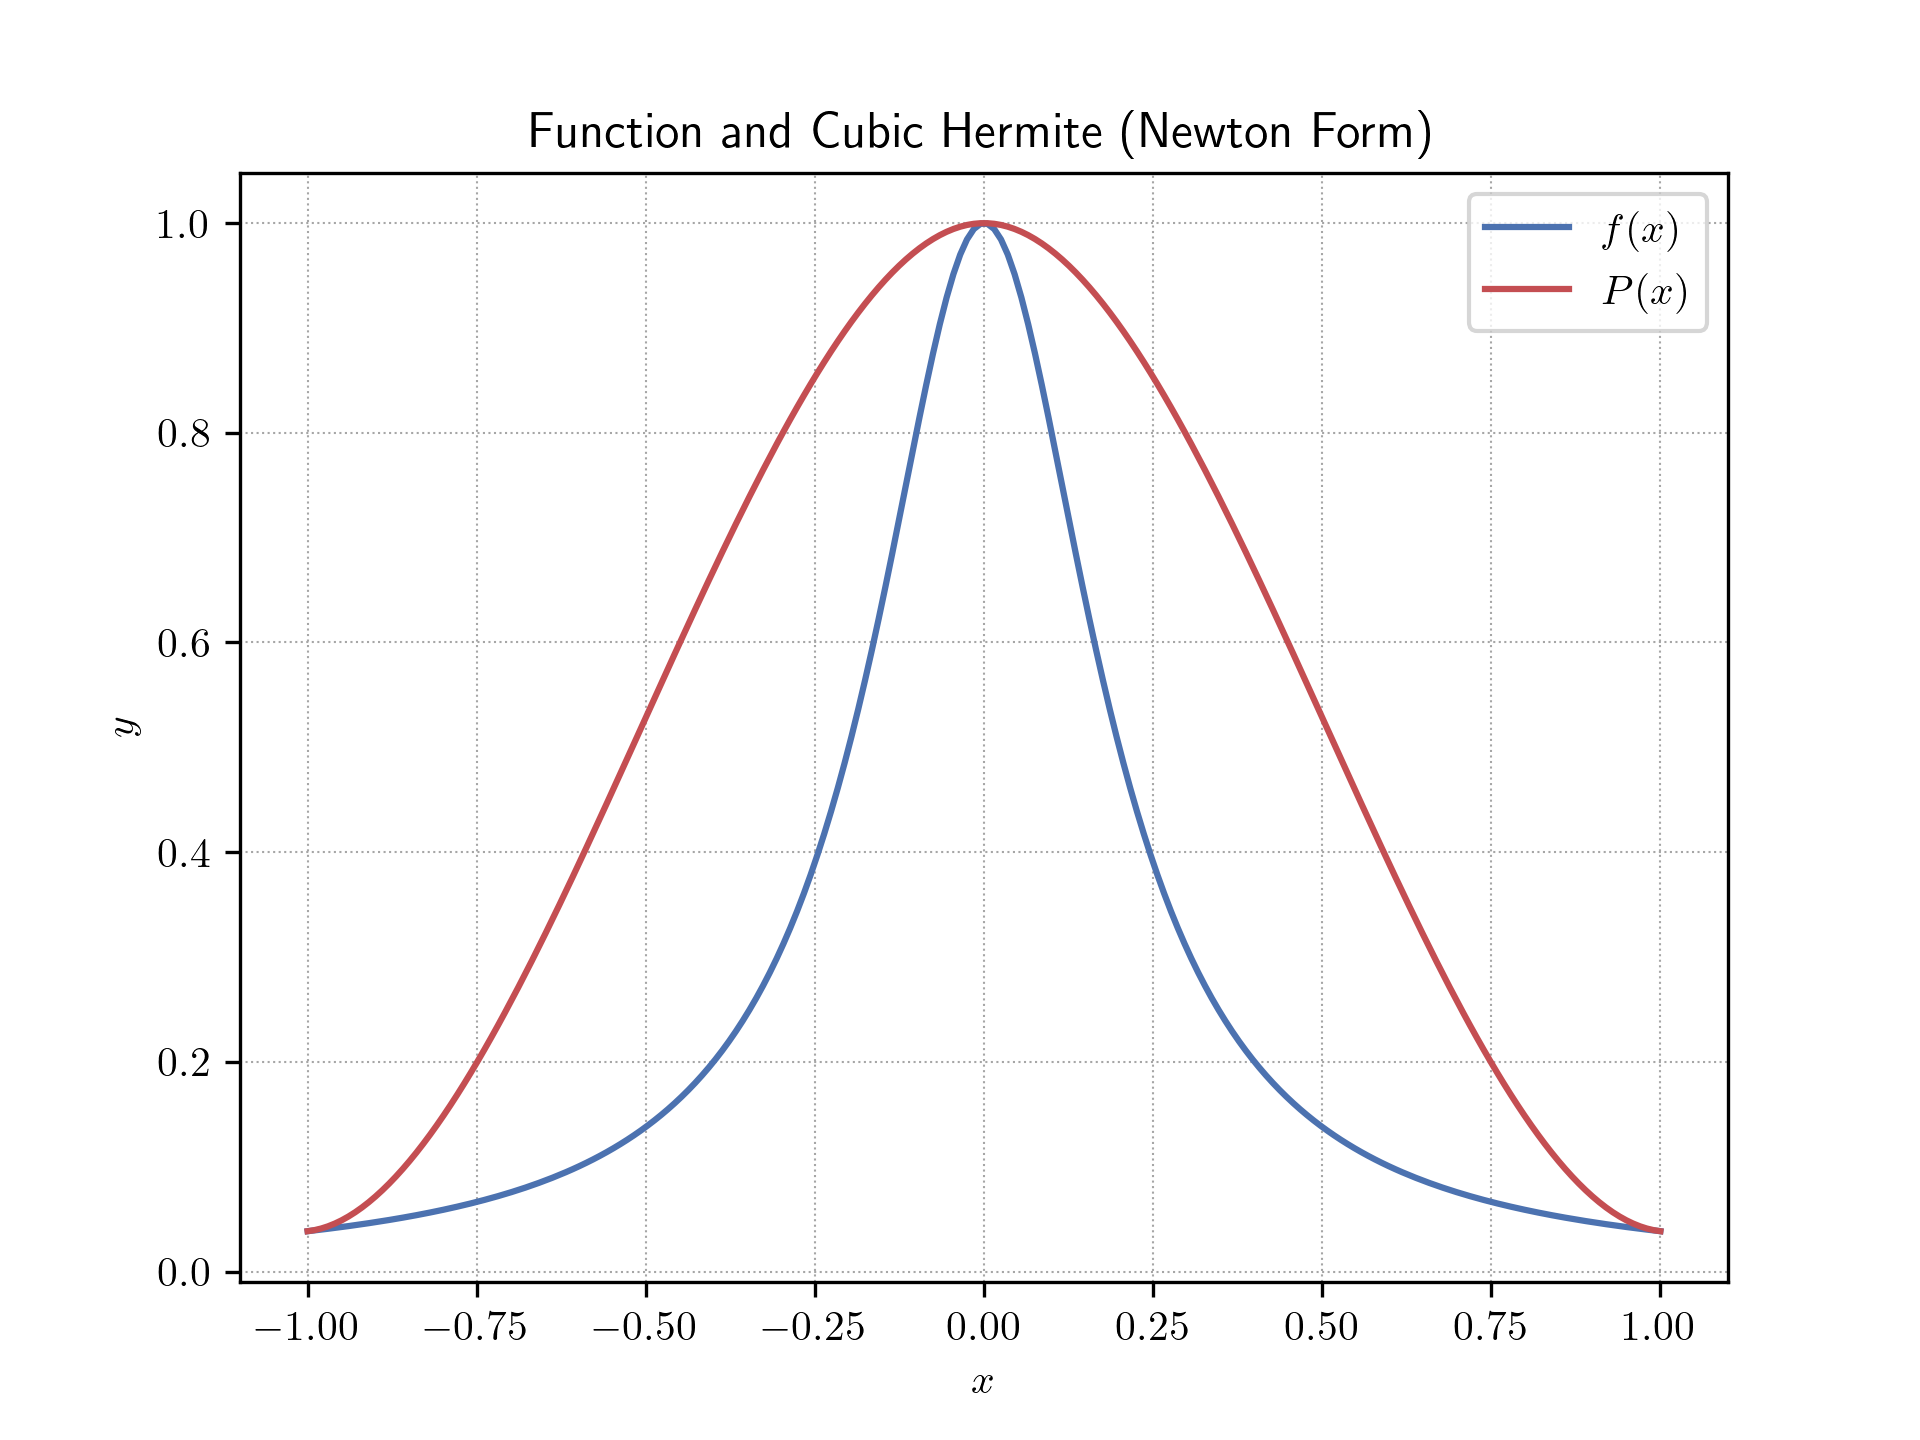
\includegraphics[width=0.7\textwidth]{../outputs_3/hermite_plot_p.png}
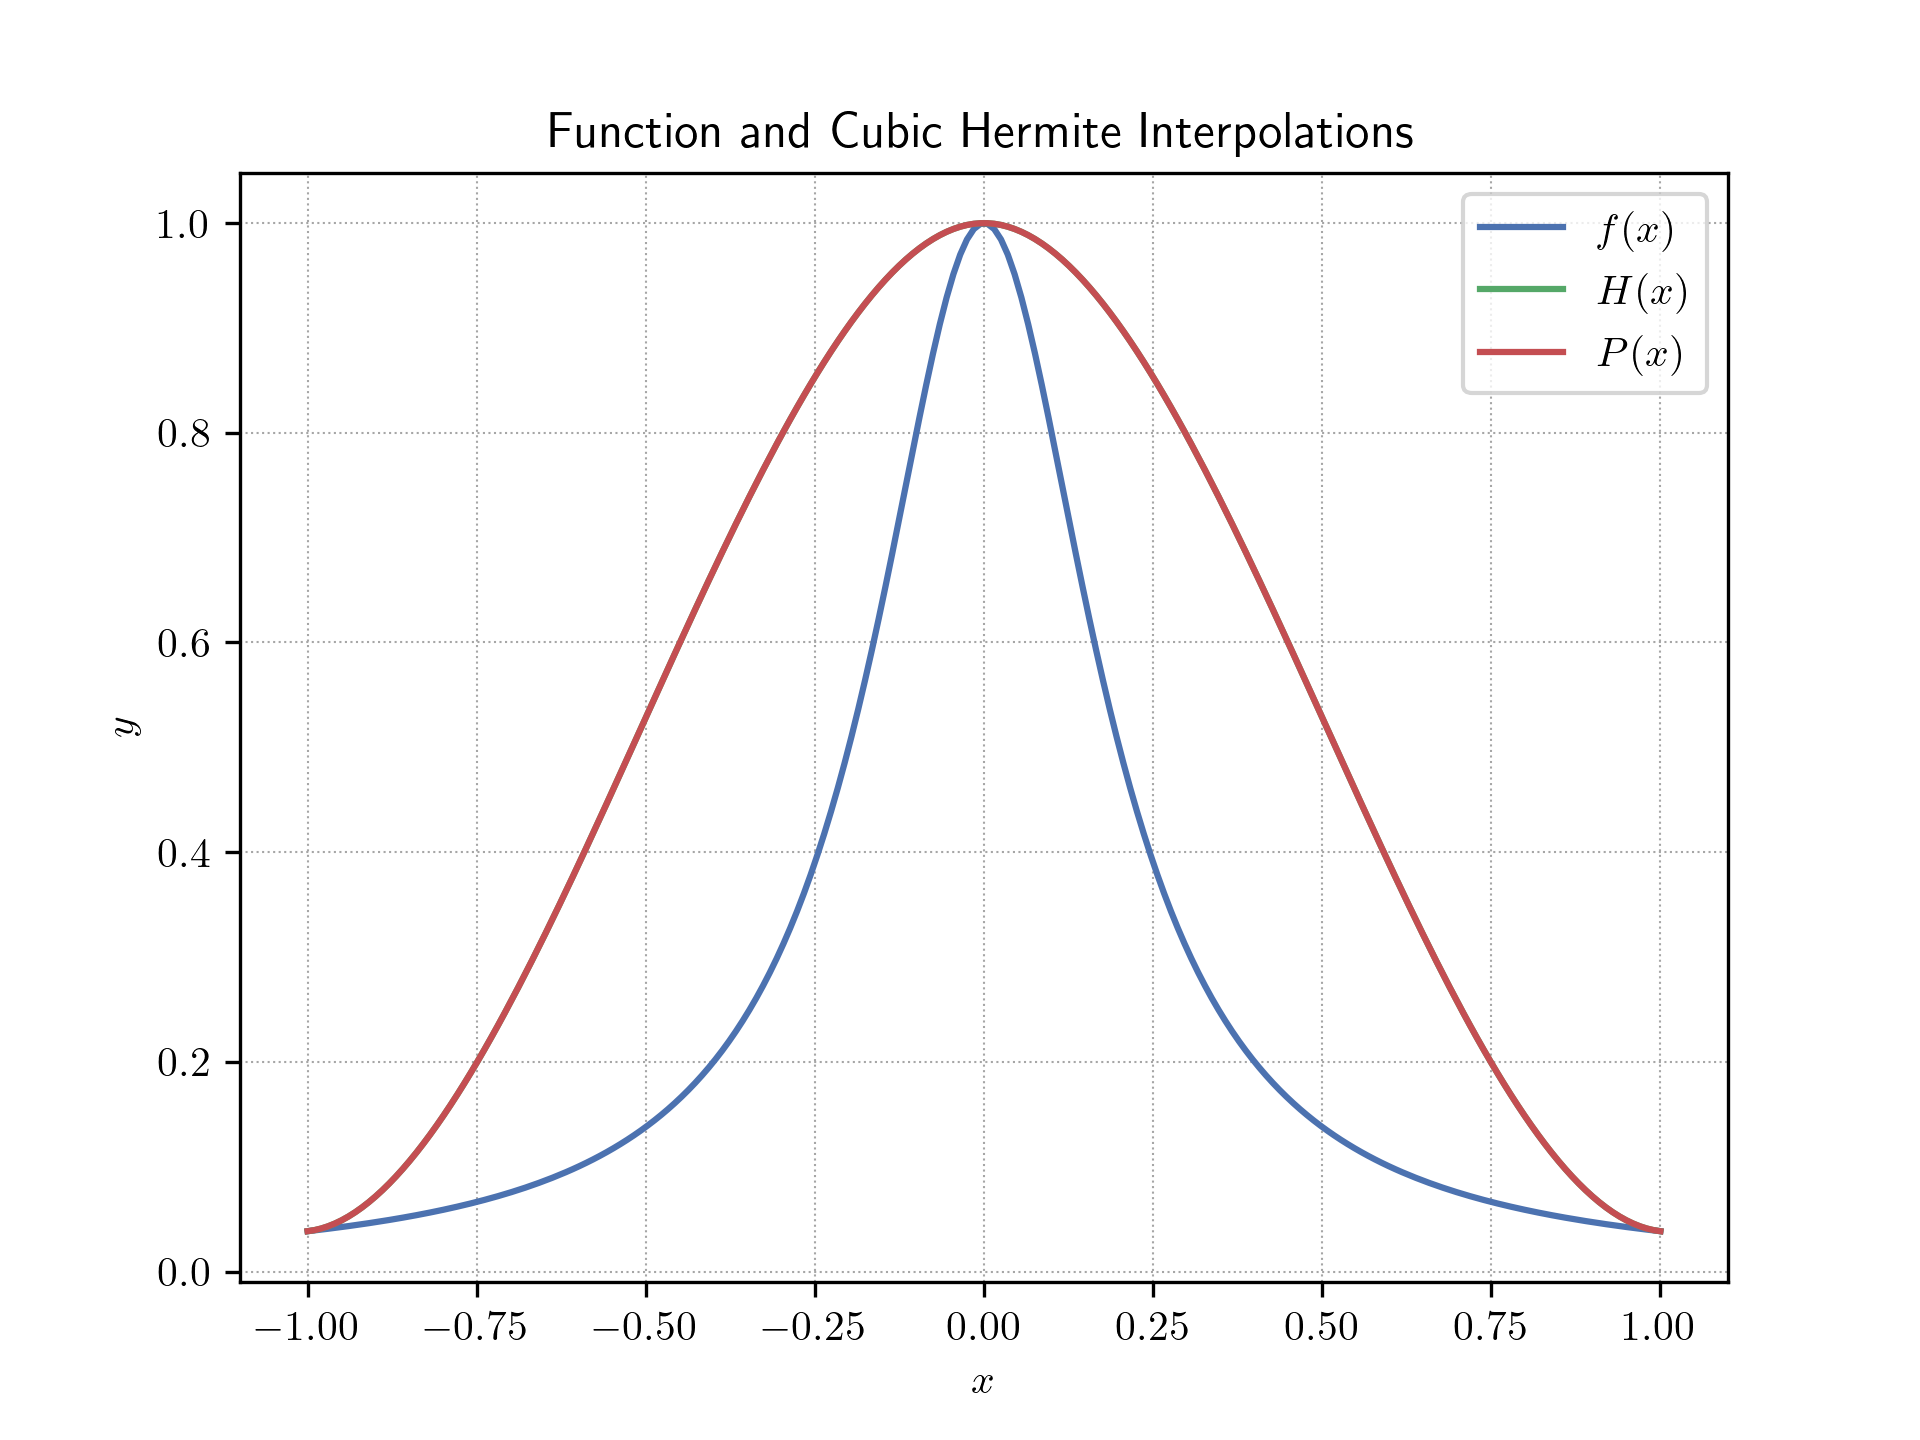
\includegraphics[width=0.7\textwidth]{../outputs_3/hermite_plot.png}
\end{center}

We observe that both Hermite interpolants $H(x)$ and $P(x)$ are identical and loosely follow the behavior of $f(x)$ on the interval $[-1,1]$.

\newpage

\question{Simple Analysis on Finite Difference}
Consider the forward difference formula for the first derivative of a smooth function $f(x)$:
\[D_hf(x) = \frac{f(x+h)-f(x)}{h}\]
The total error for this approximation can be expressed as:
\[E(h)=\frac{C_1}{h}+C_2h\]
with the optimal step size $h$:
\[h_{opt}=\sqrt{\frac{C_1}{C_2}}\]
where $C_1$ and $C_2$ are constants depending on $f(x)$, machine precision $\varepsilon$, and its derivatives.

Let $f(x) = e^x$, and take $x=1.5$.

\subquestion
Compute $f'(1.5)$ using the forward difference formula 
for a range of step sizes $h=10^{-k}$, where $k=1,2,
\ldots, 10$.

\solution
The following code was used to compute the forward difference approximations:

\begin{lstlisting}[language=Python, caption=2.1 Python]
import numpy as np

def forward_diff(f, x, step=1):
    return (f(x + step) - f(x)) / step

if __name__ == "__main__":
    with open("./outputs_3/forward_diff.txt", "w") as file:
        for k in range(1,11):
            h =10**(-k)
            f_prime = forward_diff(np.exp, 1.5, h)
            file.write(f'\\[D_h^{{({k})}}f(1.5) = {f_prime}\\]\n')
\end{lstlisting}

The following results were obtained for $D_h^{(k)}f(1.5)$:
\[D_h^{(1)}f(1.5) = 4.713433540570504\]
\[D_h^{(2)}f(1.5) = 4.5041723976187775\]
\[D_h^{(3)}f(1.5) = 4.483930662008362\]
\[D_h^{(4)}f(1.5) = 4.481913162264206\]
\[D_h^{(5)}f(1.5) = 4.4817114789097445\]
\[D_h^{(6)}f(1.5) = 4.48169131139764\]
\[D_h^{(7)}f(1.5) = 4.481689304114411\]
\[D_h^{(8)}f(1.5) = 4.481689064306238\]
\[D_h^{(9)}f(1.5) = 4.481689686031132\]
\[D_h^{(10)}f(1.5) = 4.48169501510165\]

\subquestion
Plot the absolute error $|D_hf(1)-f'(1)|$ verses $h$ 
on a log-log scale. (Report code)

\solution
The following code was used to compute and plot the absolute error:
\begin{lstlisting}[language=Python, caption=2.2 Python]
import numpy as np
import matplotlib.pyplot as plt

def calc_absolute_error(f, step, eval_x=1, diff_method=forward_diff):
    approx = diff_method(f, eval_x, step)
    return np.abs(approx - f(eval_x))

if __name__ == "__main__":
    # <Some matplotlib styling and enable LaTeX>
    h = np.logspace(-1, -10, 200)
    error = calc_absolute_error(np.exp, h)
    plt.loglog(h, error, label='$\\log|D_hf(1) - f\'(1)|$')
    plt.xlabel('$\\log(h)$')
    plt.title('Absolute Error in Forward Difference Approximation')
    plt.legend()
    plt.savefig('./outputs_3/forward_diff_graph.png', dpi=300)
    plt.show()
\end{lstlisting}

The resulting plot was:
\begin{center}
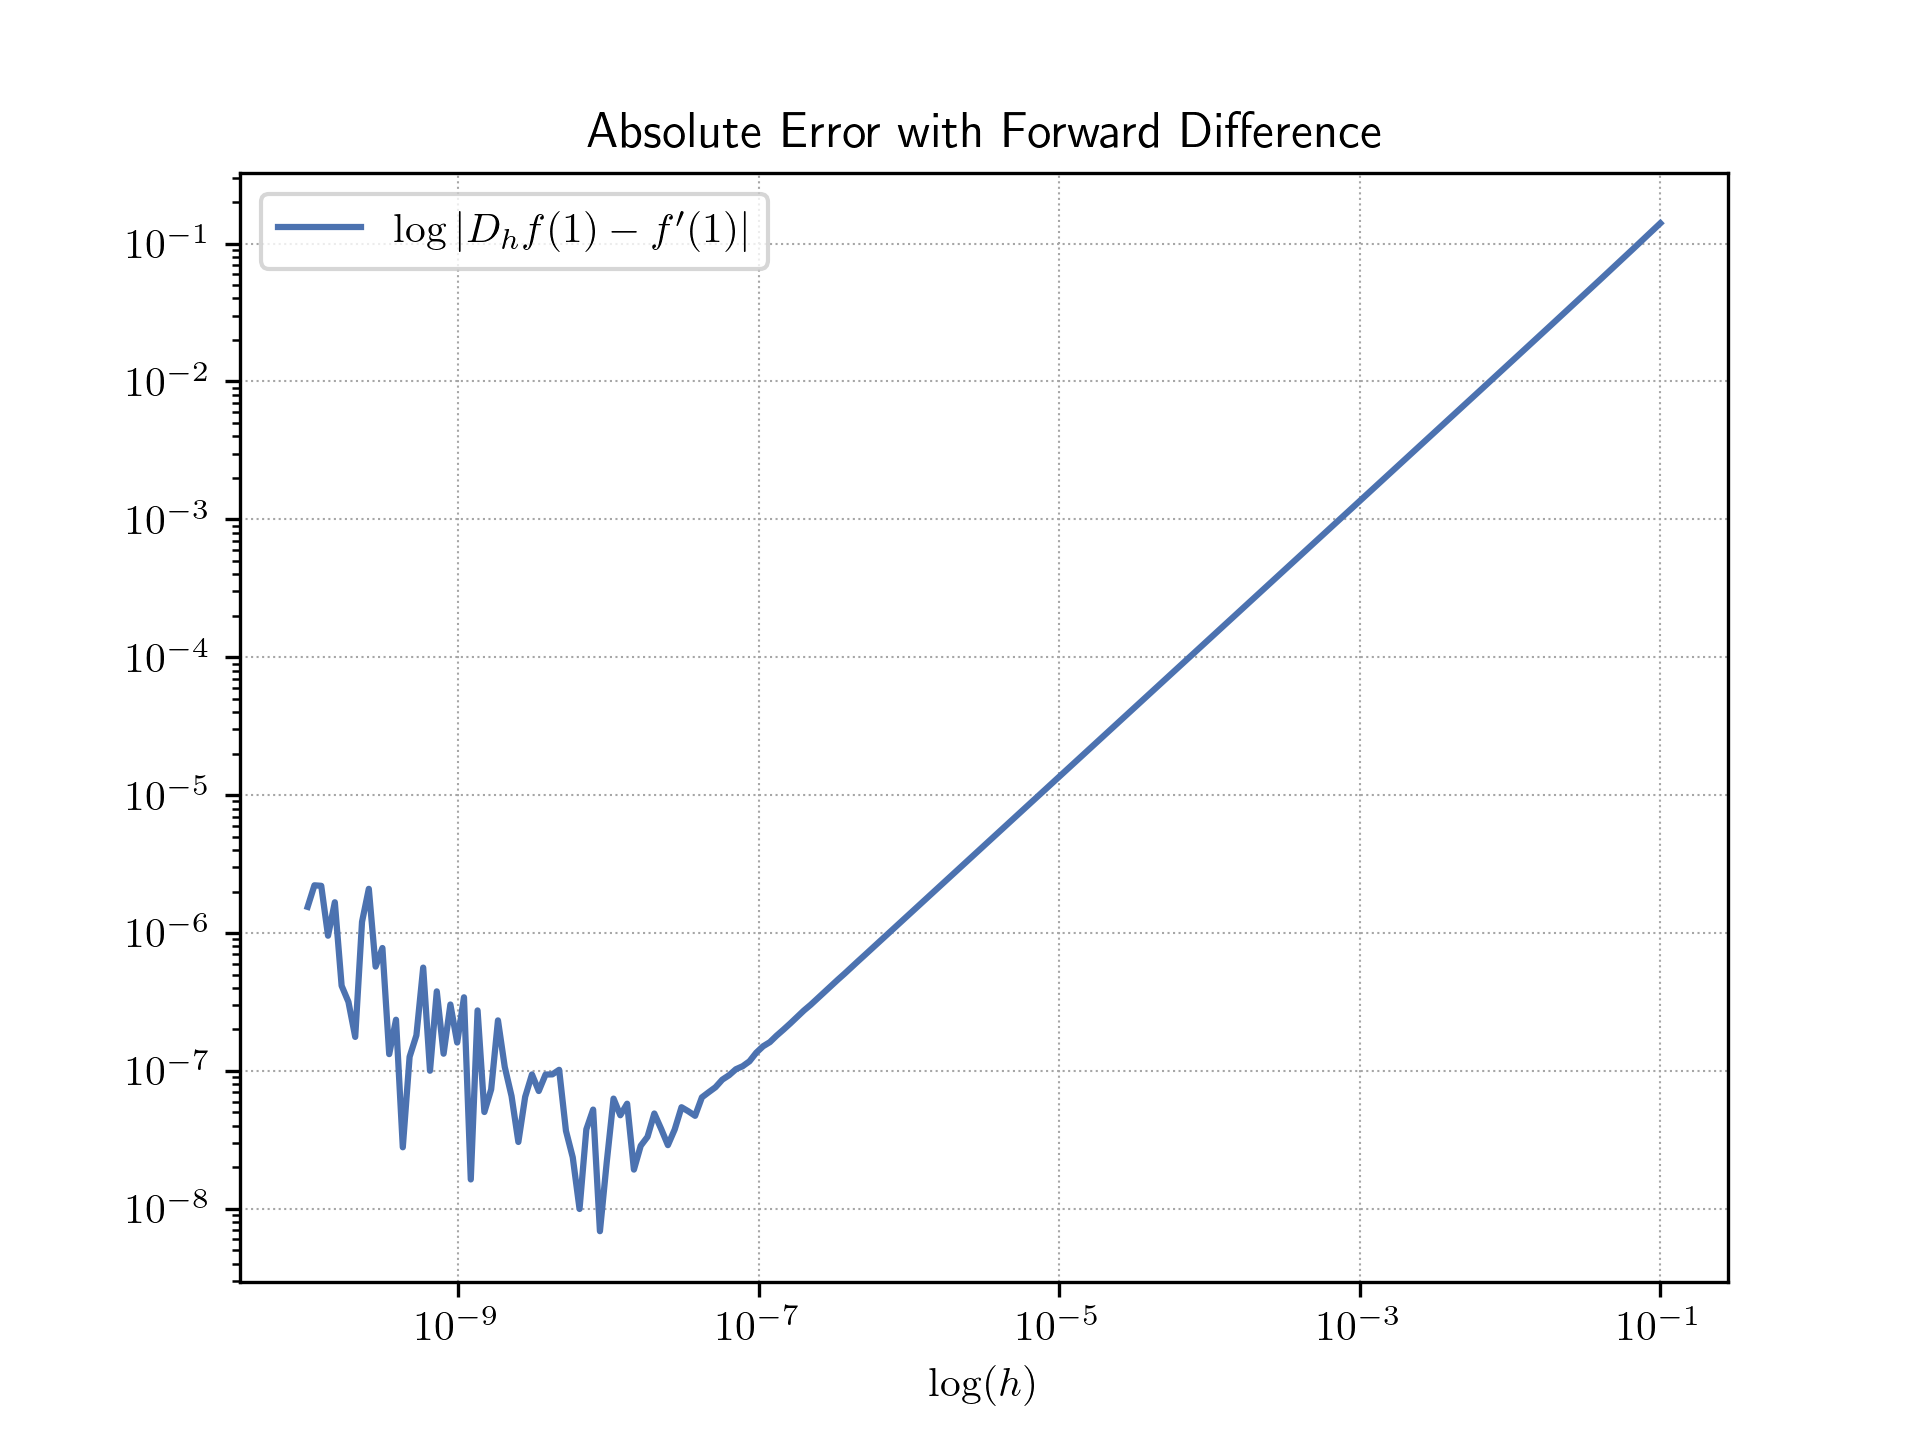
\includegraphics[width=0.7\textwidth]{../outputs_3/forward_diff_graph.png}
\end{center}

We observe that machine error starts to occur as $h$ gets smaller than approximately than $10^{-7}$.

\subquestion
Identify the $h$ that minimizes the total error and 
compare it with the predicted $h_{opt}$.

\solution
From the plot above, we observe that the minimum error occurs around $h \approx 10^{-8}$.

Machine error is $\varepsilon \sim 10^{-16}$ for double precision floating point numbers. From the notes, we have that $C_1 \sim \varepsilon |f(1)|$ and $C_2 \sim \frac{|f''(1)|}{2}$. This resulted in $h_{opt} \propto \sqrt{\varepsilon} \approx 10^{-8}$, which aligns with our observed minimum error point.

\subquestion
Use the one-sided three points scheme to approximate $f'(1.5)$, and repeat question 2.2.

\solution
The one-sided three-point finite difference formula for the first derivative is given by:
\[D_hf(x) = \frac{-3f(x) +4f(x+h) - f(x+2h)}{2h}\]

The following code was used to compute and plot the absolute error using the three-point forward difference scheme:
\begin{lstlisting}[language=Python, caption=2.4 Python]
import numpy as np 
import matplotlib.pyplot as plt

def three_point_forward_diff(f, x, step=1):
    return (-3 * f(x) + 4 * f(x + step) - f(x + 2 * step)) / (2 * step)

if __name__ == "__main__":
    # <Some matplotlib styling and enable LaTeX>
    h = np.logspace(-1, -10, 200)
    error = calc_absolute_error(np.exp, h, diff_method=three_point_forward_diff)
    
    plt.loglog(h, error, label='$\\log|D_hf(1) - f\'(1)|$')
    plt.xlabel('$\\log(h)$')
    plt.title('Absolute Error with Three Point Forward Difference')
    plt.legend()
    plt.savefig('./outputs_3/three_point_forward_diff_graph.png', dpi=300)
    plt.show()
\end{lstlisting}

The resulting plot was:
\begin{center}
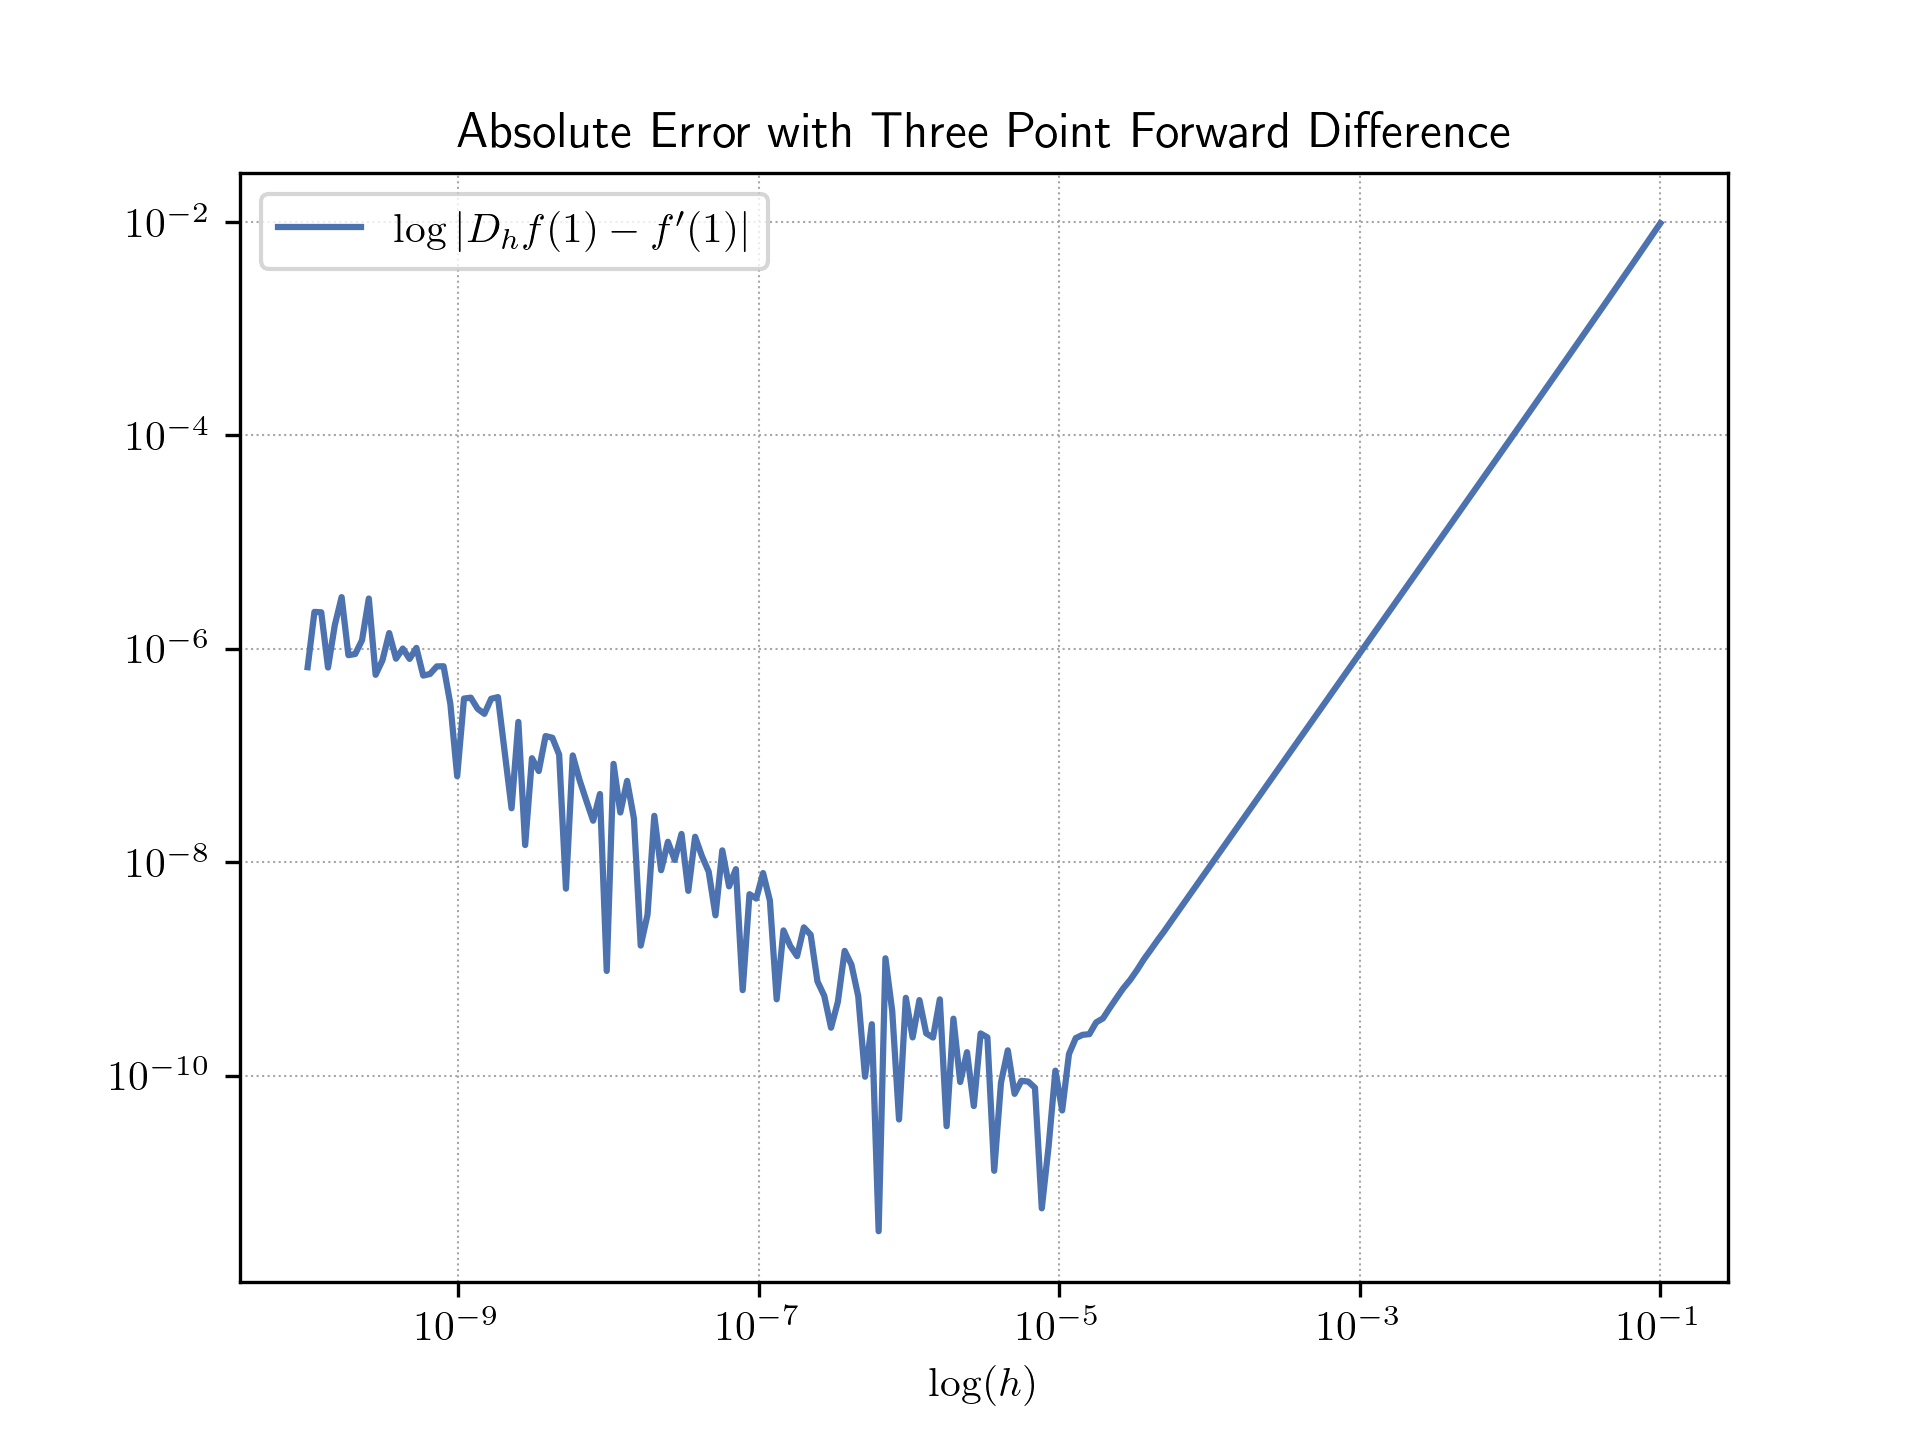
\includegraphics[width=0.7\textwidth]{../outputs_3/three_point_forward_diff_graph.png}
\end{center}

We observe that machine error starts to occur as $h$ gets smaller than approximately than $10^{-5}$.

\newpage

\question{Solve Burger's Equation by Finite Difference Scheme}
Consider the 1D viscous Burgers' equation:
\[u_t+uu_x=vu_{xx},\quad x\in[0,1], \ t>0, \ v=0.2\]
Design, analyze, and implement a numerical method that 
is stable and achieves at least second-order accuracy 
in both space and time.

\subquestion
Report finite difference scheme used.

\solution
We will be using RK4 with 2nd order finite differences for space.

First let us discretize our system. Let ${x_0, x_1, ..., x_n}$ be a partition of $[0,1]$ with step size $\Delta x =h=\frac{1}{n}$. Let $t_0, t_1, ..., t_m$ be a partition of $[0, T]$ with step size $\Delta t$. Let $u_i$ be the numerical approximation of $u(x_i, t)$.

We can construct our schemes for $u_x, u_{xx}$ from the Taylor expansion of $u$ centered at $x_i$:
\[u(x) = u(x_i) +u_x(x_i)(x-x_i) + \frac{u_{xx}(x_i)}{2}(x-x_i)^2 + \frac{u_{xxx}(x_i)}{6}(x-x_i)^3 + ...\]
Which gives us for $x=x_i - h$ and $x=x_i + h$:
\[u(x_i-h) = u(x_i) - hu_x(x_i) + \frac{h^2}{2}u_{xx}(x_i) - \frac{h^3}{6}u_{xxx}(x_i) + O(h^4)\]
\[u(x_i+h) = u(x_i) + hu_x(x_i) + \frac{h^2}{2}u_{xx}(x_i) + \frac{h^3}{6}u_{xxx}(x_i) + O(h^4)\]

Approximate $u_x$ centrally by:
\[u(x_i+h)-u(x_i-h) = 2hu_x(x_i) + O(h^3)\]
Which gives us the second-order scheme:
\[u_x(x_i) \approx \frac{u(x_i+h) - u(x_i - h)}{2h} + O(h^2)\]

Approximate $u_{xx}$ with the usual second-order central difference:
\[u(x_i+h) - 2u(x_i) + u(x_i - h) = h^2u_{xx}(x_i) + O(h^4)\]
Which gives us the second-order scheme:
\[u_{xx}(x_i) \approx \frac{u(x_i+h) - 2u(x_i) + u(x_i - h)}{h^2} + O(h^2)\]

Rearranging Burger's equation for $u_t$, we have:
\[u_t = -uu_x + vu_{xx}\]
Substituting in our finite difference approximations, we obtain the ODE:
\[\frac{d u_i}{dt} \approx -u_i \cdot \frac{u_{i+1}- u_{i-1}}{2h} + v \cdot \frac{u_{i+1} - 2u_i + u_{i-1}}{h^2}+O(h^2)\]
Which is $O(h^2)=O(\Delta x^2)$ accurate in space. Denote the right-hand side above as $F(u_i)$. 

More compactly, write the system as:
\[\frac{d u}{dt} = F(u) + O(\Delta x^2)\]
Where $u = [u_0, u_1, ..., u_n]^T$.

We will now use RK4 to approximate $u^{n+1}$, which is given by:
\[u^{n+1} = u^n + \frac{\Delta t}{6}(k_1 + 2k_2 + 2k_3 + k_4)\]
Such that:
\[k_1 = F(u^n)\]
\[k_2 = F\left(u^n + \frac{\Delta t}{2}k_1\right)\]
\[k_3 = F\left(u^n + \frac{\Delta t}{2}k_2\right)\]
\[k_4 = F\left(u^n + \Delta t k_3\right)\]

RK4 is $O(\Delta t^4)$ accurate in time, so our overall scheme is $O(\Delta t^4)+O(\Delta x^2)$.
We also note that RK4 would have CFL conditions for stability:
\[\Delta t \leq \frac{C_1 \Delta x}{\max |u|}, \quad \Delta t \leq \frac{C_2 \Delta x^2}{v}\] 
Where $C_1, C_2$ are constants depending on the scheme.
In practice, we can choose $\Delta t$ based on the more restrictive of the two conditions above and pick smaller $C_1, C_2$ to be safe.

\subquestion
Use the initial condition as a sine wave $\sin(2\pi x)$. 
Implement the scheme and plot the numerical solution 
at $T=1 \text{ second}$.

\solution
We have Burger's equation:
\[u_t+uu_x=vu_{xx},\quad x\in[0,1], \ t>0, \ v=0.2\]
With periodic initial condition:
\[u(x,0) = \sin(2\pi x)\]
This means that $u(0,t) = u(1,t)$ for all $t \geq 0$. Since our data is periodic, no extra scheme is needed for the boundaries and we can just treat $u$ as a circular array.

The following code was used to implement the scheme:
\begin{lstlisting}[language=Python, caption=3.2 Python]
import numpy as np
import matplotlib.pyplot as plt
from copy import deepcopy

def initial_condition(x):
    return np.sin(2 * np.pi * x)

def rk4_step(u, dt, dx, v):
    def F(u):
        # Compute spatial derivatives using central differences
        u_x = (np.roll(u, -1) - np.roll(u, 1)) / (2 * dx)
        u_xx = (np.roll(u, -1) - 2 * u + np.roll(u, 1)) / (dx**2)
        return -u * u_x + v * u_xx

    k1 = F(u)
    k2 = F(u + 0.5 * dt * k1)
    k3 = F(u + 0.5 * dt * k2)
    k4 = F(u + dt * k3)

    return u + (dt / 6) * (k1 + 2 * k2 + 2 * k3 + k4)

def burgers_rk4(dx, t_final, v=0.2, start_x=0, end_x=1, return_history=False):
    # Take ceil for num_nodes
    num_nodes = int((end_x - start_x) / dx) + 1
    x = np.linspace(start_x, end_x, num_nodes)
    
    # The CFL condition for diffusion is more restrictive
    # as for initial condition u = sin(2pi x), max|u| = 1
    # Pick C_2 = 0.5 to be safe
    dt = 0.5 * dx**2 / v
    num_time_steps = int(np.ceil(t_final / dt))
    # Adjust dt to fit exactly into t_final
    dt = t_final / num_time_steps  

    u = initial_condition(x)

    # Store history of u for Question 3.4
    if return_history:
        t = 0
        u_history = [deepcopy(u)]
        times = [t]

    for _ in range(num_time_steps):
        u = rk4_step(u, dt, dx, v)
        if return_history:
            t += dt
            u_history.append(deepcopy(u))
            times.append(t)
            
    if return_history:
        return x, u, np.array(times), np.array(u_history)
    
    return x, u

if __name__ == "__main__":
    dx = 1e-1
    t_final = 1
    x, u = burgers_rk4(dx, t_final)
    
    # <Some matplotlib styling and enable LaTeX>

    plt.plot(x, u, label=f'$u(x, {t_final})$')
    plt.title("1D Burgers' Equation with RK4")
    plt.xlabel("$x$")
    plt.legend()
    plt.savefig('./outputs_3/burgers_rk4.png', dpi=300)
    plt.show()
\end{lstlisting}

The resulting plot at $T=1$ second was:
\begin{center}
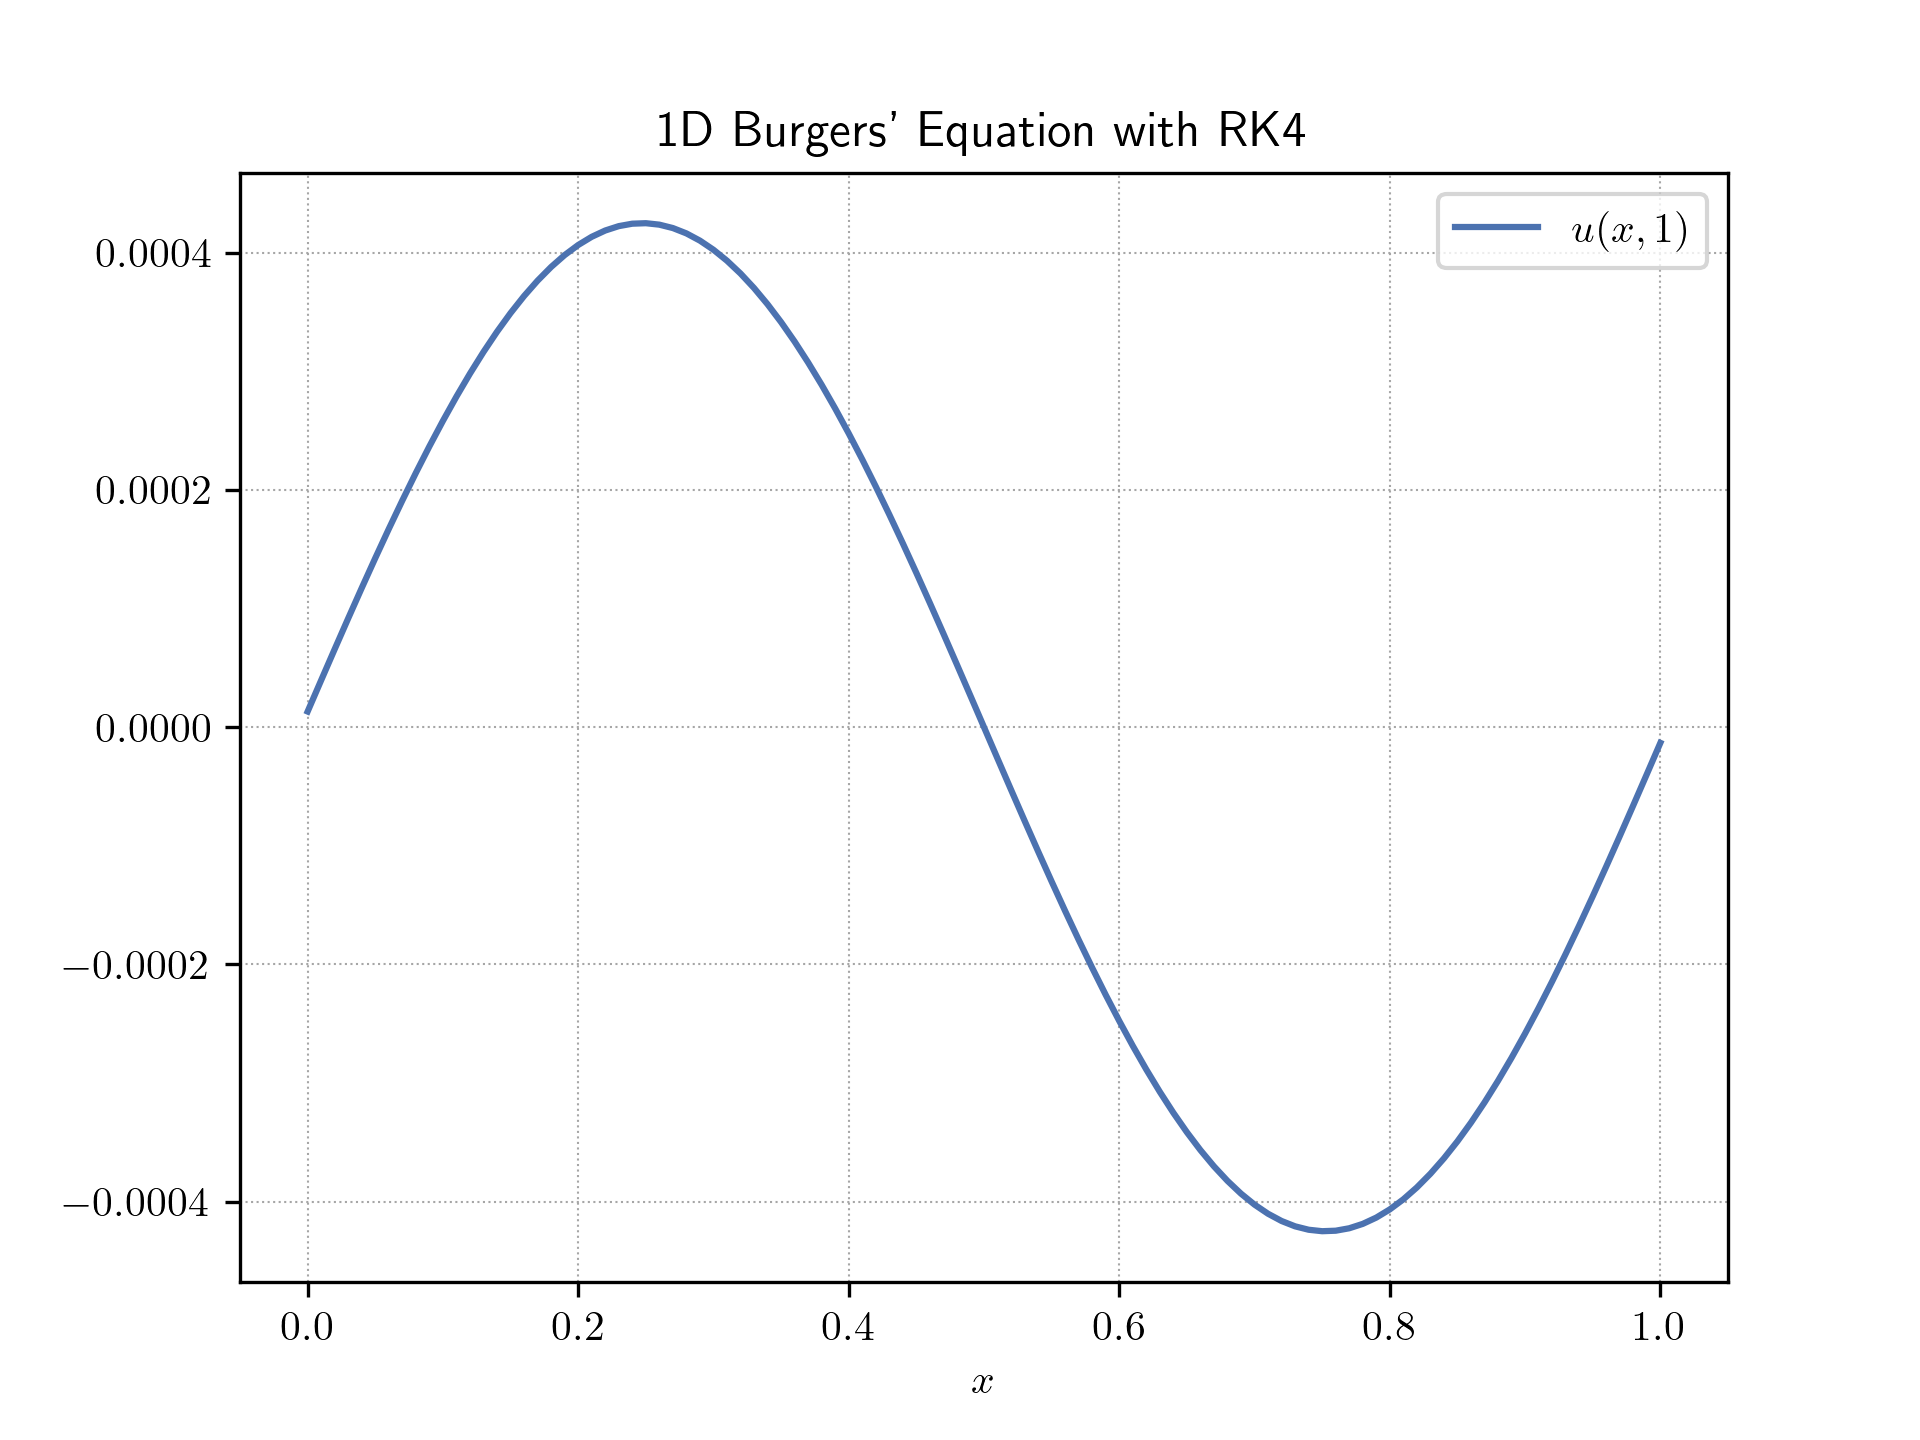
\includegraphics[width=0.7\textwidth]{../outputs_3/burgers_rk4.png}
\end{center}


\subquestion
Compute $||u-u_h||_{L^2}$ with a different refined 
mesh, and show your spatial convergence in a log-log
plot.

\solution
The discrete $L^2$ norm was used to compute our error:
\[||u - u_h||_{L^2} = \sqrt{\Delta x \sum_{i=1}^{N}(u_i - u_{h,i})^2}\]
Where $N$ is the number of spatial nodes in the coarser mesh, $u_i$ is the exact solution at node $i$, and $u_{h,i}$ is the numerical solution at node $i$.

The following code was used to compute the $L^2$ error and plot spatial convergence:
\begin{lstlisting}[language=Python, caption=3.3 Python]
import numpy as np
import matplotlib.pyplot as plt

def discrete_l2(u_num, u_ref, dx):
    return np.sqrt(np.sum((u_num - u_ref)**2) * dx)

def spacial_convergence(dx_list, t_final, v=0.2):
    
    # dx_exact will serve as our "exact" solution
    # Use a finer dx than minimum dx in dx_list
    dx_exact = min(dx_list) / 4
    x_exact, u_exact = burgers_rk4(dx_exact, t_final, v)
    
    errors = []
    for dx in dx_list:
        x_approx, u_approx = burgers_rk4(dx, t_final, v)
        # Interpolate exact solution to the current mesh of x_approx
        u_exact_on_x_approx = np.interp(x_approx, x_exact, u_exact)
        error = discrete_l2(u_approx, u_exact_on_x_approx, dx)
        errors.append(error)
    return dx_list, errors

if __name__ == "__main__":
    # <Some matplotlib styling and enable LaTeX>
    dx_list = np.logspace(-2, -9, 18, base=2)
    dx, error = spacial_convergence(dx_list, t_final)
    plt.loglog(dx, error, label='$||u - u_h||_{L^2}$')
    plt.xlabel('$\\log(\\Delta x)$')
    plt.title('L2 Error vs Spatial Step Size')
    plt.legend()
    plt.savefig('./outputs_3/burgers_rk4_error.png', dpi=300)
    plt.show()
\end{lstlisting}

The plot generated for spatial convergence at $T=1$ was:
\begin{center}
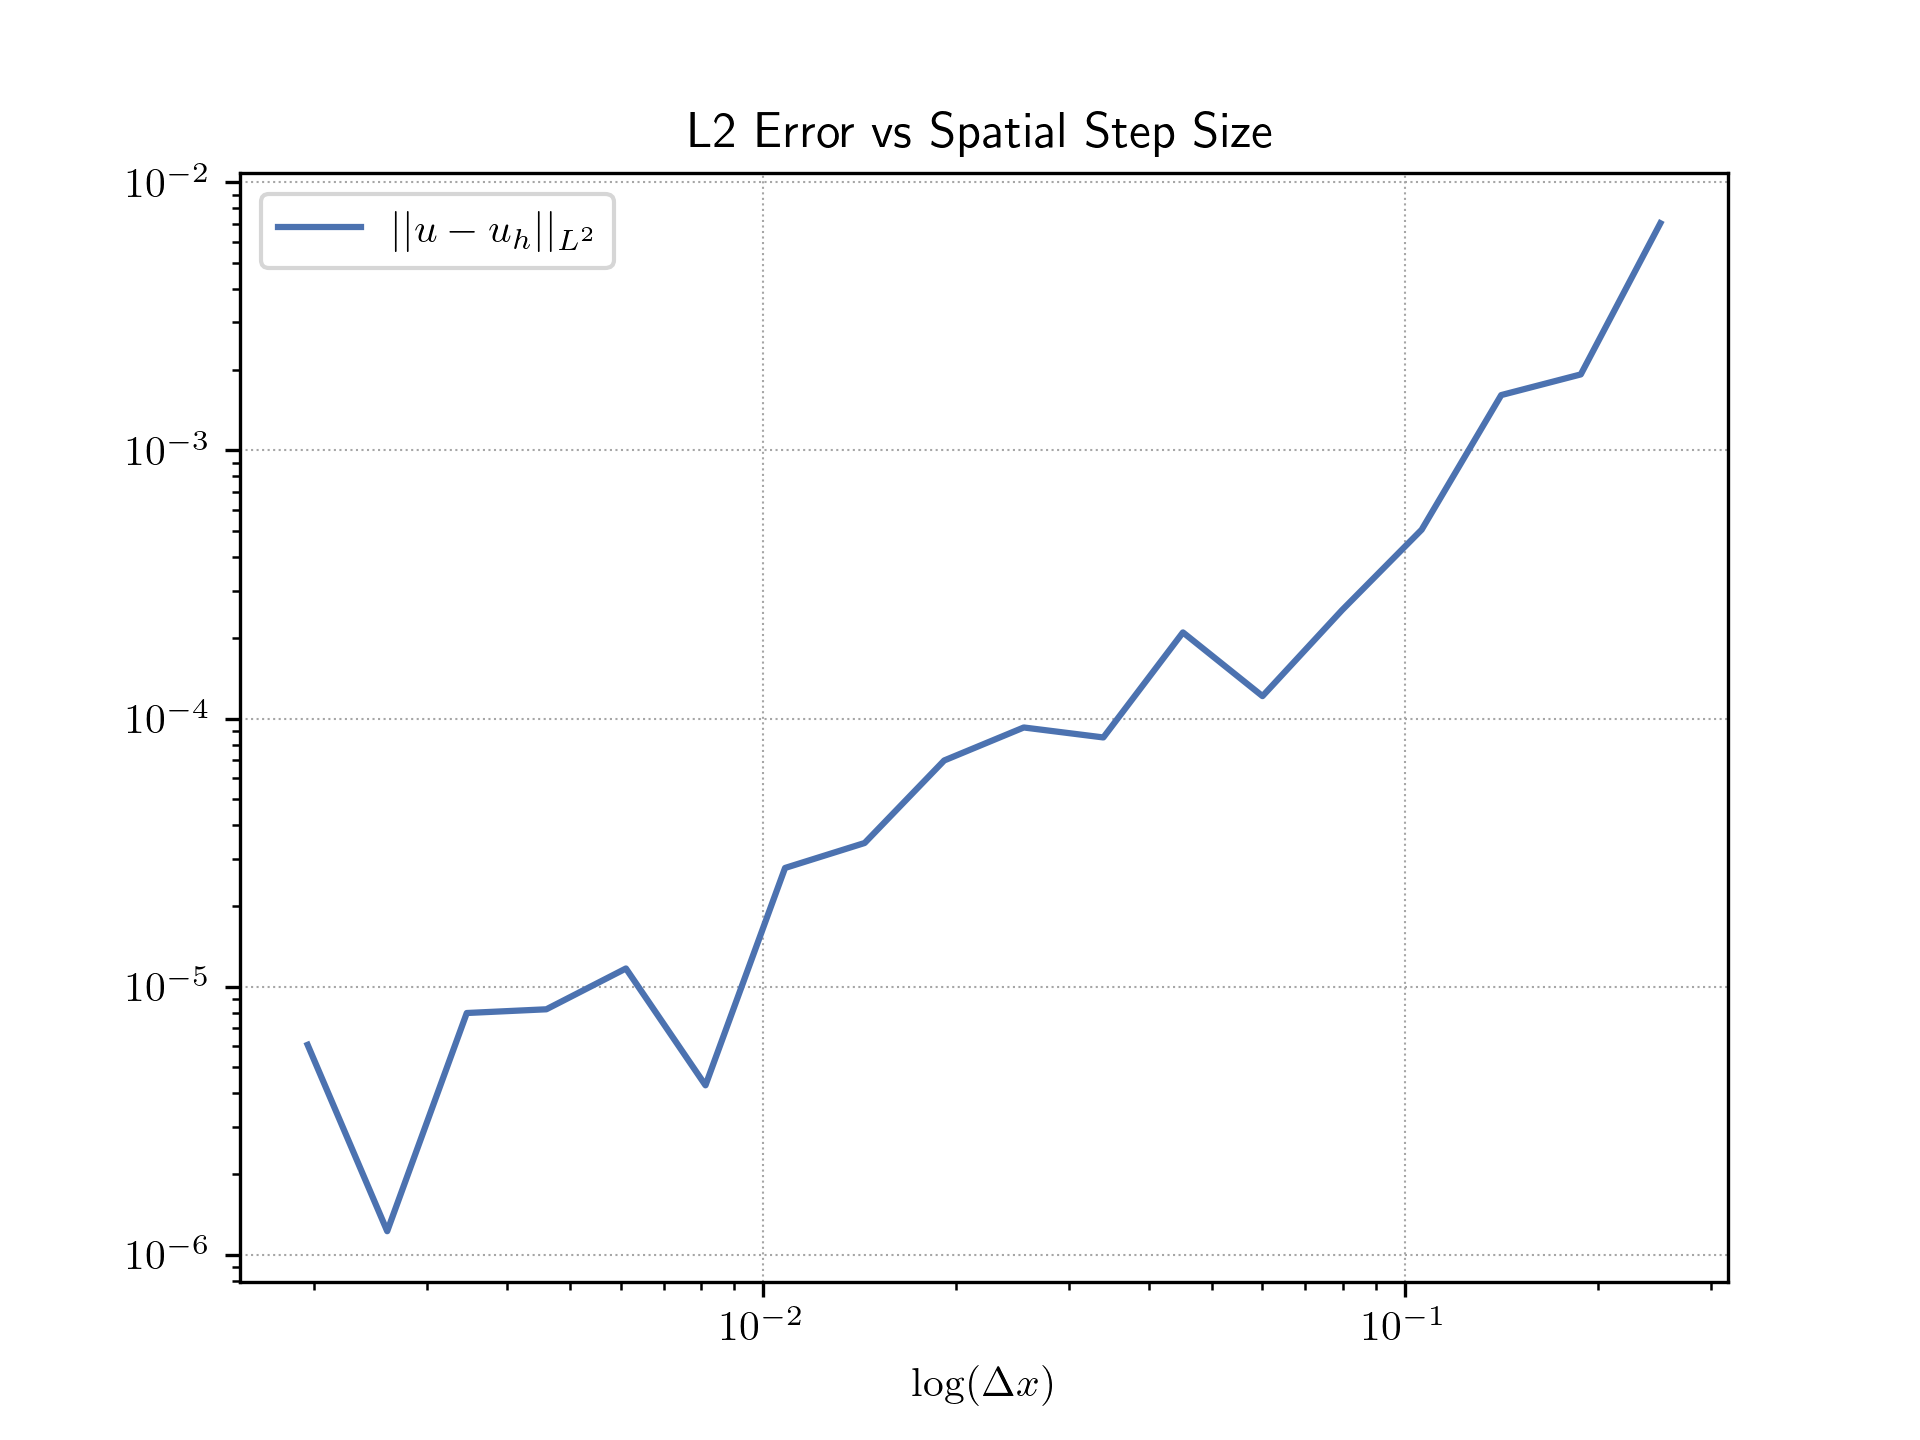
\includegraphics[width=0.7\textwidth]{../outputs_3/burgers_rk4_error.png}
\end{center}

A few notes:
\begin{enumerate}
    \item $\Delta x=\frac{1}{2}$ has been excluded from the plot as it had favorable error due to the coarse mesh aligning well with the sine wave at $T=1$.
    \item The fluctuations in the error can be explained by additional interpolation error when mapping the exact solution to the coarser mesh and/or point 1 above.
\end{enumerate}

Overall, we observe second-order spatial convergence as $\Delta x$ decreases.

\subquestion
Plot your $||u-u_h||_{L^2}$ vs time.

\solution
The following code was used to compute and plot the $L^2$ error vs time:
\begin{lstlisting}[language=Python, caption=3.4 Python]
import numpy as np
import matplotlib.pyplot as plt

def norm_vs_time(dx, t_final, x_exact, u_exact_history, v=0.2):
    x_approx, _, times, u_history = burgers_rk4(dx, t_final, v, return_history=True)
    
    norms = []
    for u_approx, u_exact in zip(u_history, u_exact_history):
        u_exact_on_x_approx = np.interp(x_approx, x_exact, u_exact)
        norm = discrete_l2(u_approx, u_exact_on_x_approx, dx)
        norms.append(norm)
    return times, norms

if __name__ == "__main__":
    # <Some matplotlib styling and enable LaTeX>
    dx_list = np.logspace(-2, -6, 5, base=2)

    dx_exact = min(dx_list) / 4
    x_exact, _, _, u_exact_history = burgers_rk4(dx_exact, t_final, return_history=True)

    for index, dx in enumerate(dx_list):
        time, norms = norm_vs_time(dx, t_final, x_exact, u_exact_history)
        plt.plot(time, norms, label=f'$h = 2^{{{-index-2}}}$')
    plt.xlabel('$t$')
    plt.ylabel(r'$||u - u_h||_{L^2}$')
    plt.title('L2 Error vs Time')
    plt.legend()
    plt.savefig('./outputs_3/burgers_rk4_error_vs_time.png', dpi=300)
    plt.show()
\end{lstlisting}

The plot generated for $L^2$ error vs time was:
\begin{center}
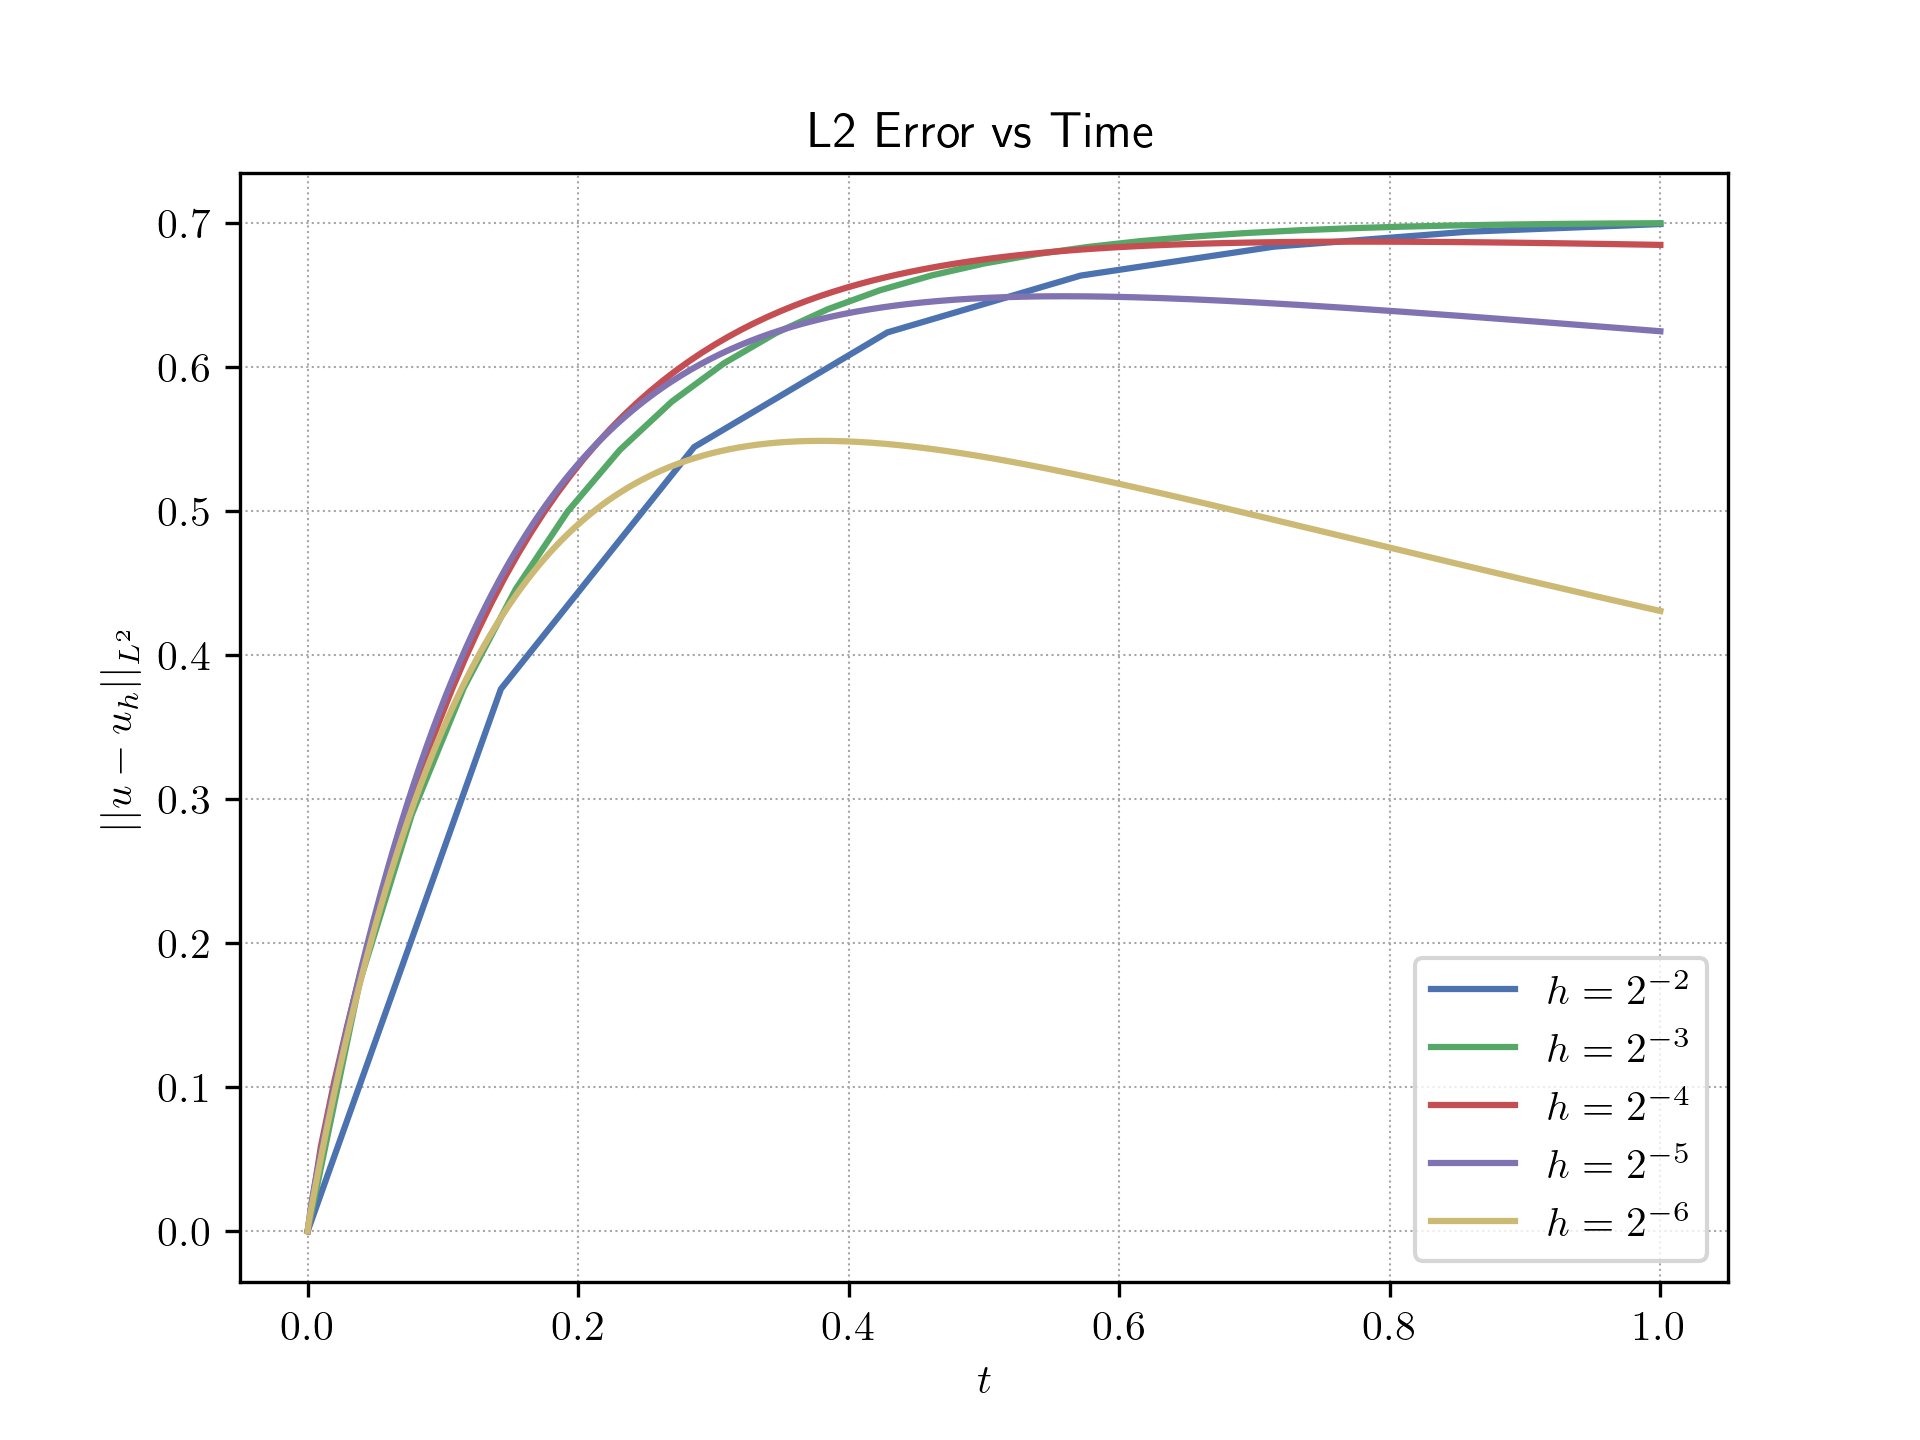
\includegraphics[width=0.7\textwidth]{../outputs_3/burgers_rk4_error_vs_time.png}
\end{center}

We can see that the $L^2$ error generally increases with time and then stabilizes. The increase makes sense as numerical errors accumulate over time steps.
 
Finer meshes (smaller $h$) consistently yield lower errors throughout the simulation at $T=1$.

\end{document}